\chapter{UI / UX}
\label{ch:ui-ux}

Two distinct experiences must be described: the experience of the \emph{tool}
(terminal and editor) and the experience of the \emph{generated screens}.

\section{Tool experience --- terminal}

\begin{longtable}{@{}L{4cm}L{10.2cm}@{}}
\caption{Terminal interaction design}\\
\toprule
\textbf{Element} & \textbf{Design} \\
\midrule
\endfirsthead
\toprule
\textbf{Element} & \textbf{Design} \\
\midrule
\endhead
Colour semantics & Cyan for informational headings
(\texttt{Generating "Login Screen" (auth/login)...}), green for success
(\texttt{\checkmark Login Screen added successfully!}), yellow for warnings and
notices, red for errors, dim grey for secondary detail (the effective options line,
the registry source line, skipped files). \\
Progressive disclosure & Options are asked for only when they cannot be resolved. \\
Defaults & Prompts preselect the detected value when the recipe supports it. \\
Filtering & Prompts list only the values the recipe supports. \\
Confirmation & The effective option set is printed before generation:
\texttt{styling=... router=... ui=... icons=... typescript=...}. \\
Per-file feedback & Each written file is announced as \texttt{Created
<path>}. \\
Follow-up guidance & Three concrete next steps after generation. \\
Safe abort & Any handled error leaves the exit code at 1 and writes nothing further. \\
\bottomrule
\end{longtable}

\section{Tool experience --- VS Code}

\begin{longtable}{@{}L{4cm}L{10.2cm}@{}}
\caption{Editor interaction design}\\
\toprule
\textbf{Element} & \textbf{Design} \\
\midrule
\endfirsthead
\toprule
\textbf{Element} & \textbf{Design} \\
\midrule
\endhead
Discoverability & Three entry points (completion, command palette, status bar) so the
tool is reachable without reading documentation. \\
Inline trigger & The trigger regex matches only immediately before the cursor
(\texttt{snip:} or \texttt{expo-snips:}), so ordinary typing does not spam the
completion list. \\
Completion items & Labelled with the recipe id (the thing the user must type),
detailed with the display name, documented with the description and tags, sorted by
id. \\
Non-destructive insert & The completion inserts no text; selecting it runs the
generation command instead. This avoids leaving stray trigger text in the file. \\
Selection & Quick Pick matches on label and description
(\texttt{matchOnDescription: true}). \\
Progress & A progress notification covers the write phase. \\
Completion feedback & An information message reports the recipe name and file count,
and the message detail lists every generated path. \\
Follow-up action & A single ``Open main file'' button keeps the next step one click
away. \\
Empty catalog & A dedicated error message with an ``Open Settings'' action that
deep-links to the \texttt{expo-snips.registryUrl} setting. \\
\bottomrule
\end{longtable}

\section{Generated screen experience}

The generated screens share a consistent interaction vocabulary. The following is
observed across the templates.

\subsection*{States}

\begin{longtable}{@{}L{4cm}L{10.2cm}@{}}
\caption{States provided by generated screens}\\
\toprule
\textbf{State} & \textbf{Where and how} \\
\midrule
\endfirsthead
\toprule
\textbf{State} & \textbf{Where and how} \\
\midrule
\endhead
Loading & \texttt{isLoading} in \texttt{useLogin}/\texttt{useRegister}; a
\texttt{ActivityIndicator} is rendered in the native form. \\
Validation error & Per-field error text under the input, from
\texttt{formState.errors}. \\
Submission error & \texttt{error} state returned by the auth hooks plus
\texttt{Alert.alert}. \\
Empty & \texttt{utility/empty} --- icon, message and a primary action. \\
Error / retry & \texttt{utility/error} --- warning icon, message and a retry action. \\
Refresh & \texttt{app/home} wires a \texttt{RefreshControl} (its handler logs
\texttt{'refresh'}). \\
Unread indicator & \texttt{app/notifications} distinguishes read/unread and offers a
mark-all-read action. \\
Selected / unselected & \texttt{onboarding/features} cards and
\texttt{ecommerce} product cards. \\
\bottomrule
\end{longtable}

\subsection*{Input and validation patterns}

\begin{itemize}
  \item Controlled inputs through \texttt{react-hook-form}'s \texttt{Controller}.
  \item Email fields set \texttt{keyboardType="email-address"} and
        \texttt{autoCapitalize="none"}.
  \item Password fields combine a secure entry toggle with
        \texttt{secureTextEntry}.
  \item The OTP recipe uses a segmented input with auto-advance and auto-submit on
        completion and an error message plus a resend affordance.
  \item Labels are rendered above the field in the native variant; the shadcn
        variant instead pairs an icon with a borderless input inside a row.
\end{itemize}

\subsection*{Navigation patterns}

\begin{itemize}
  \item Expo Router screens use \texttt{Link} with route strings
        (\texttt{/register}, \texttt{/forgot-password}, \texttt{/}).
  \item The react-navigation login and register screens use
        \texttt{useNavigation()} and \texttt{navigation.goBack()}.
  \item Back affordances are a left chevron or an arrow-left icon inside a
        pressable, consistent with the surrounding palette.
\end{itemize}

\section{Visual reference --- committed screenshots}

\textbf{Status: IMPLEMENTED.} The repository ships real renders of the
generated screens. Twenty-two PNGs live in \texttt{docs/screenshots/} --- one
per screen recipe (21) plus a shot of the gallery screen used during capture.
Each image is 780\,$\times$\,1688 px (a 390\,$\times$\,844 viewport at
2$\times$ scale, light mode) and was produced by generating the screen with the
CLI (\texttt{--styling stylesheet --router expo-router --ui native --icons
lucide --typescript}) into a scratch Expo application and capturing the running
app in a headless browser. Provenance and regeneration instructions are in
\texttt{docs/screenshots/README.md}; the root \texttt{README.md} embeds the
same images in a Screen Showcase gallery. Figures~\ref{fig:shot-login}
to~\ref{fig:shot-gallery} reproduce a representative subset.

\begin{figure}[H]
    \centering
    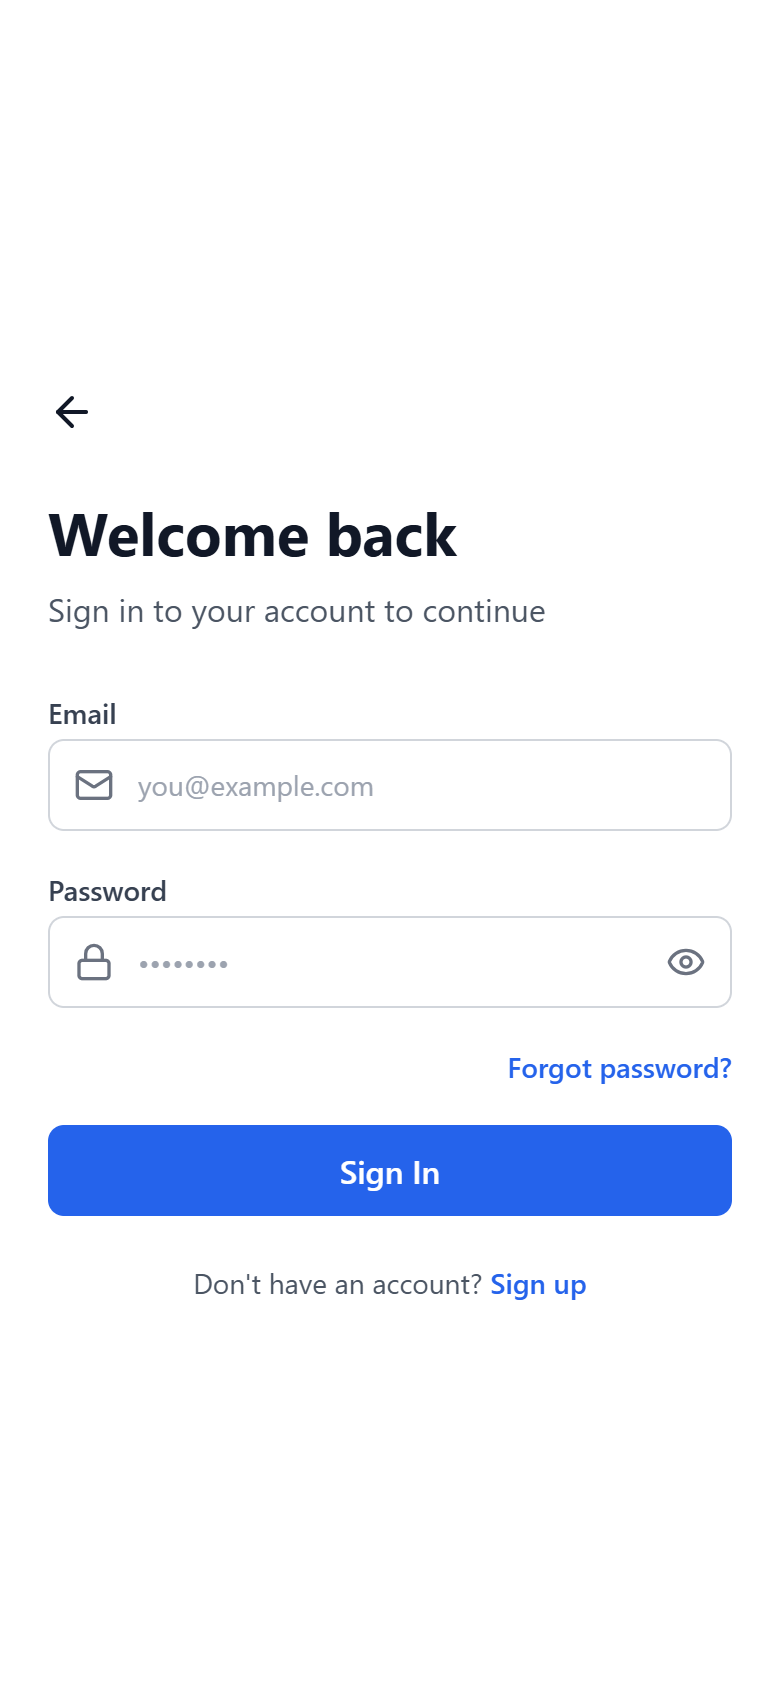
\includegraphics[width=0.36\textwidth]{assets/auth-login.png}
    \caption{Generated \texttt{auth/login} screen (screenshot from \texttt{docs/screenshots/auth-login.png}): labelled fields, icon adornments, inline links and a full-width primary button.}
    \label{fig:shot-login}
\end{figure}

\begin{figure}[H]
    \centering
    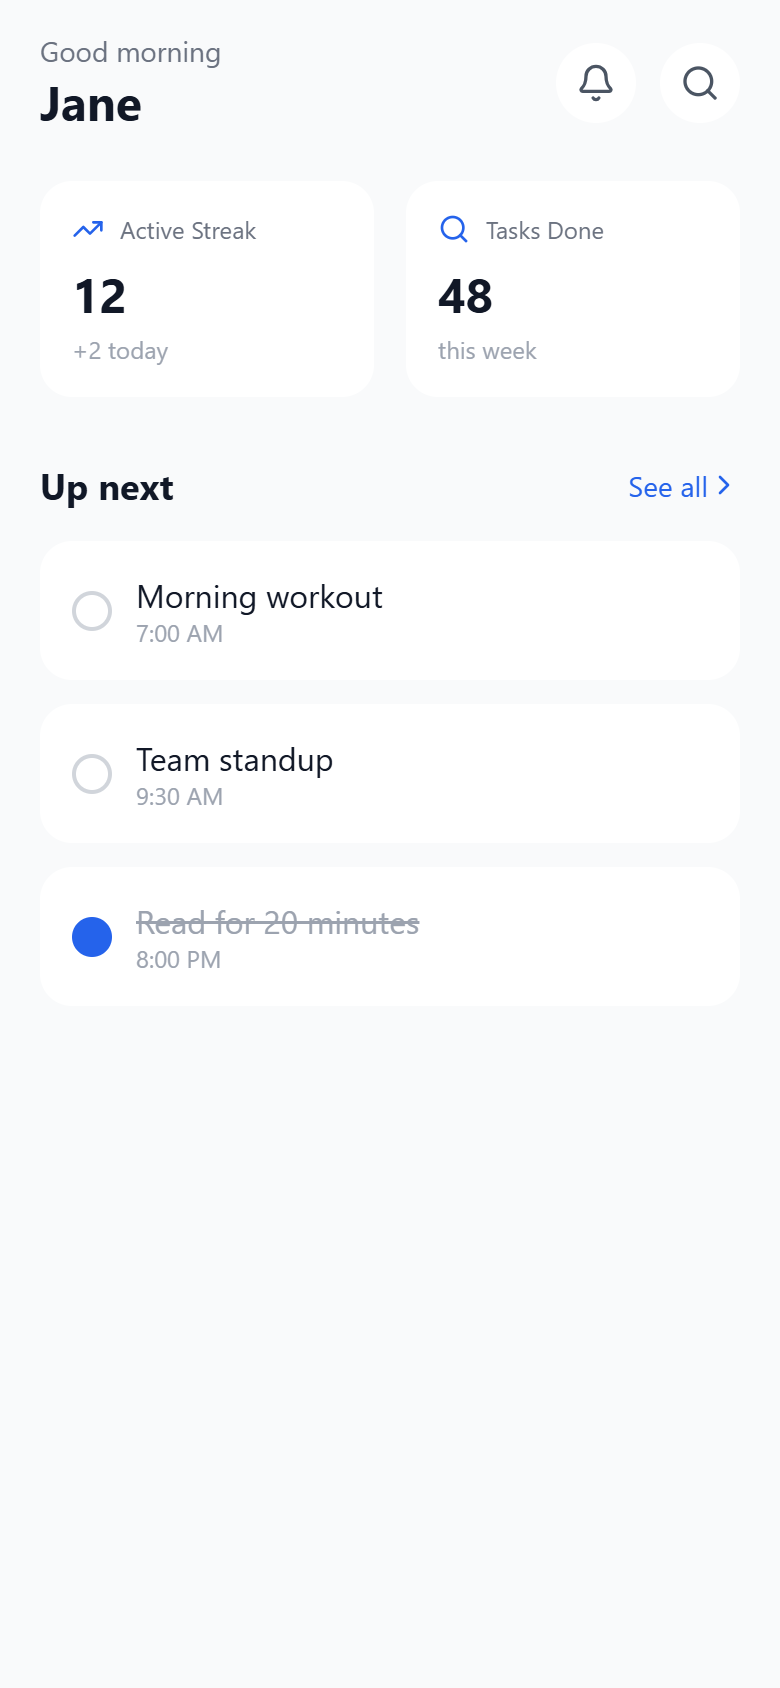
\includegraphics[width=0.36\textwidth]{assets/app-home.png}
    \caption{Generated \texttt{app/home} screen: greeting header with icon actions, stat cards and a task list with completion states.}
    \label{fig:shot-home}
\end{figure}

\begin{figure}[H]
    \centering
    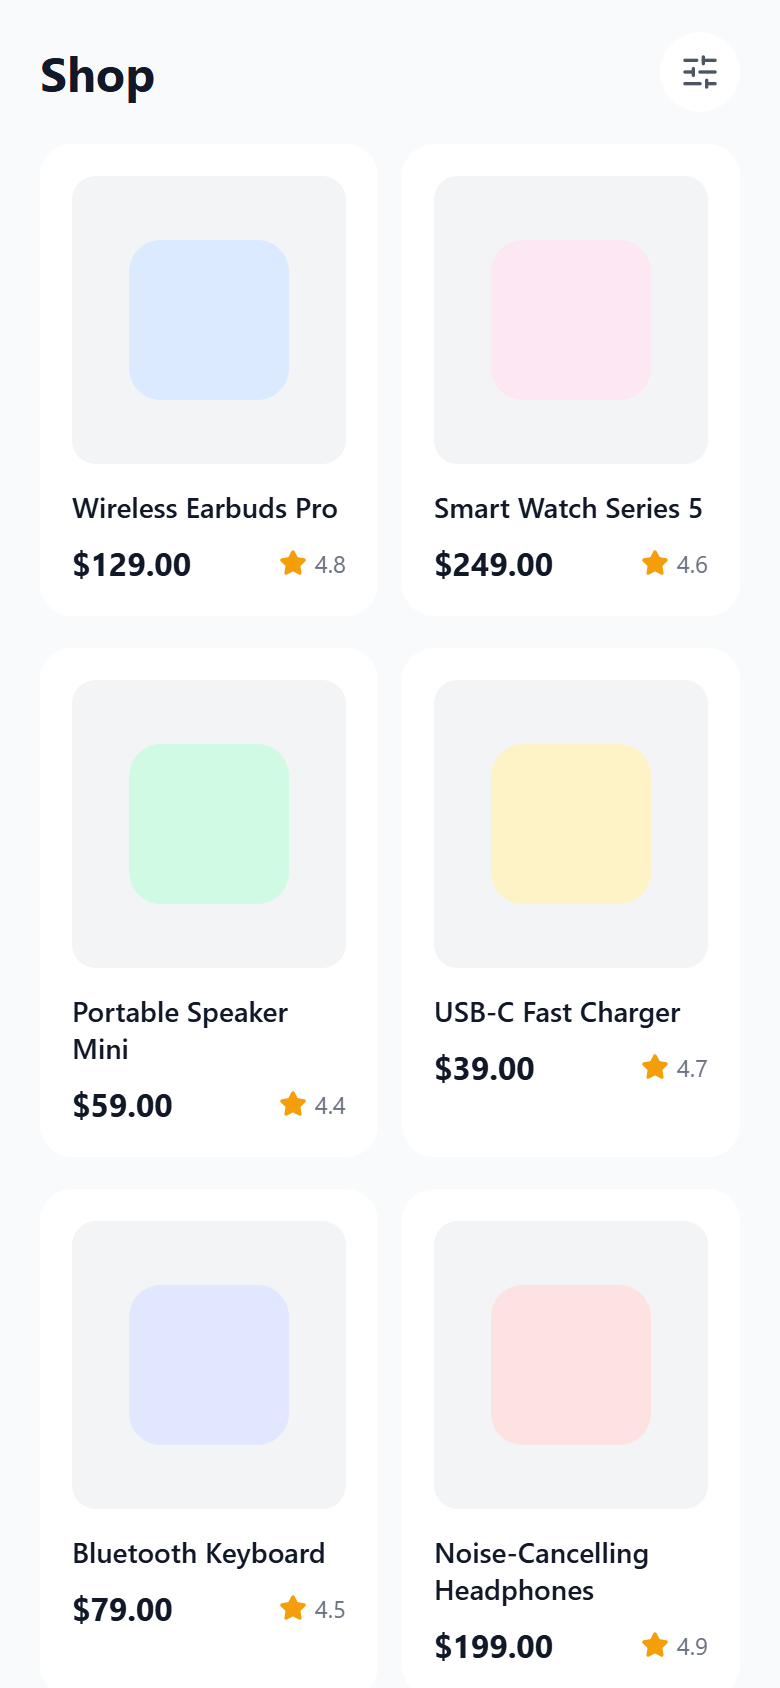
\includegraphics[width=0.36\textwidth]{assets/ecommerce-products.png}
    \caption{Generated \texttt{ecommerce/products} screen: two-column product grid with imagery, price and rating rows.}
    \label{fig:shot-products}
\end{figure}

\begin{figure}[H]
    \centering
    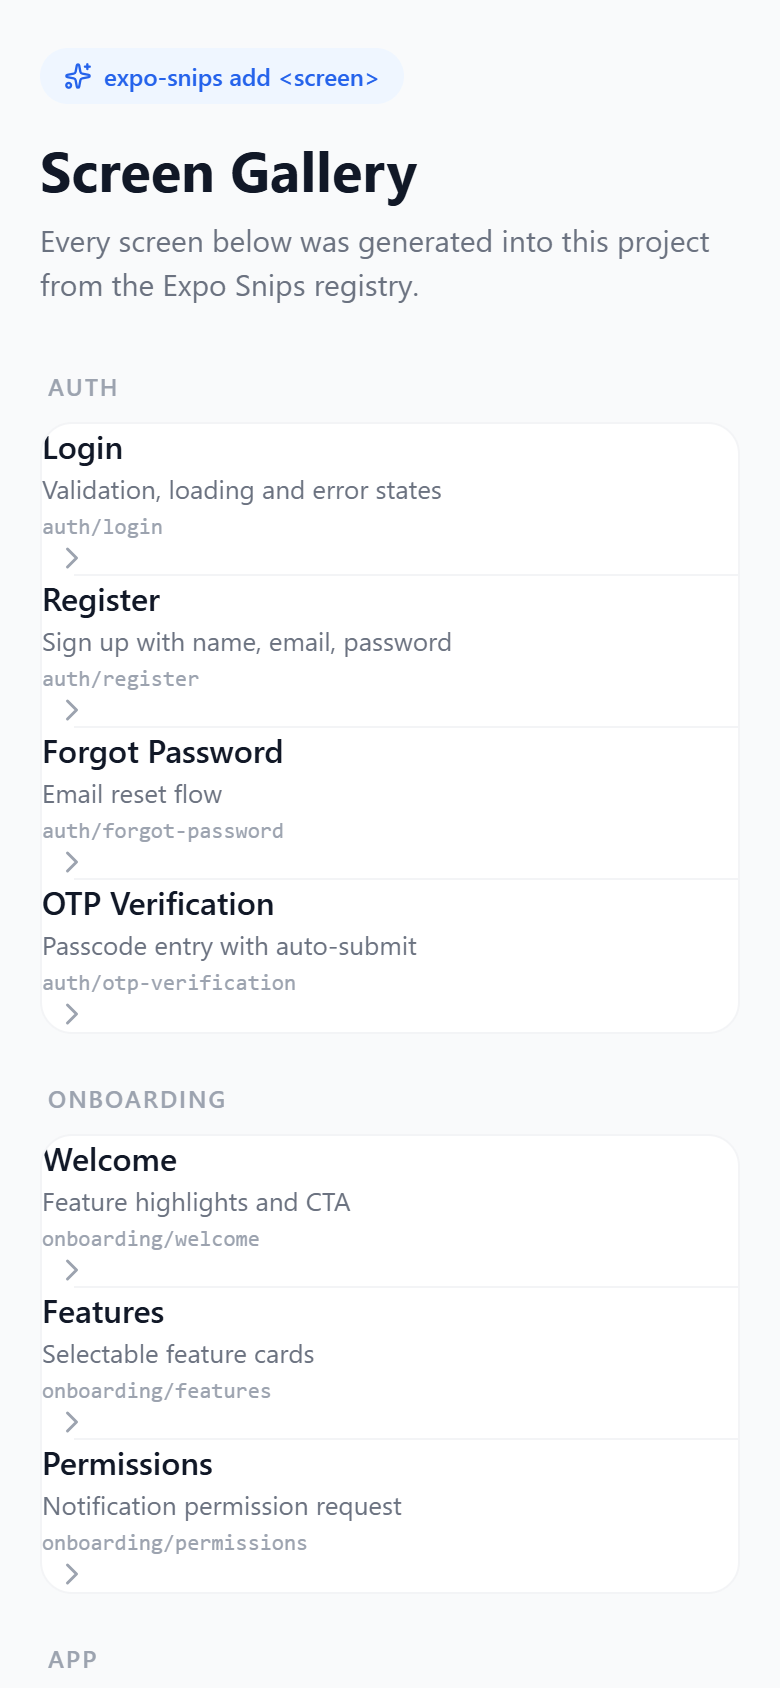
\includegraphics[width=0.36\textwidth]{assets/gallery.png}
    \caption{Gallery screen used during capture: a grouped, tappable index of every generated screen.}
    \label{fig:shot-gallery}
\end{figure}

\section{Responsive design}

All layouts use flex containers and percentage/flex sizing rather than fixed
widths, so they adapt to phone and tablet. Concrete evidence:

\begin{itemize}
  \item \texttt{ecommerce/products} uses a two-column \texttt{FlatList} grid.
  \item \texttt{app/home} uses \texttt{flex-1} stat cards in a row.
  \item Forms are wrapped in a \texttt{ScrollView} with
        \texttt{keyboardShouldPersistTaps="handled"} and a
        \texttt{KeyboardAvoidingView} whose behaviour switches on platform
        (\texttt{padding} on iOS, \texttt{height} on Android).
  \item Lists use \texttt{react-native-safe-area-context}'s \texttt{SafeAreaView}
        in some templates and React Native's own \texttt{SafeAreaView} in others ---
        an inconsistency recorded in Chapter~\ref{ch:technical-debt}.
\end{itemize}

\section{Animations and interaction feedback}

\begin{itemize}
  \item The use of \texttt{Pressable} provides the platform's native press
        feedback.
  \item The shadcn-style \texttt{Button} adds opacity changes on press
        (\texttt{active:opacity-90}) and web-only hover/focus ring behaviour.
  \item No template uses \texttt{Animated}, \texttt{Reanimated},
        \texttt{Moti} or layout transitions.
\end{itemize}

\textbf{Status:} IMPLEMENTED (as an observed absence of animation).

\section{Accessibility}

\textbf{Finding.} No generated template sets
\texttt{accessibilityLabel}, \texttt{accessibilityRole},
\texttt{accessibilityHint} or \texttt{accessibilityState}. Interactive elements are
\texttt{Pressable}s and \texttt{TextInput}s without labels for assistive
technology. Icon-only buttons (for example the header bell, search and back
buttons) expose no text alternative.

\begin{longtable}{@{}L{1.4cm}L{4.4cm}L{3cm}L{5.4cm}@{}}
\caption{Accessibility finding}\\
\toprule
\textbf{ID} & \textbf{Finding} & \textbf{Severity} & \textbf{Evidence} \\
\midrule
\endfirsthead
\toprule
\textbf{ID} & \textbf{Finding} & \textbf{Severity} & \textbf{Evidence} \\
\midrule
\endhead
A11Y-01 & Icon-only pressables have no accessibility label. & Medium & Every template with an icon button, e.g. \texttt{app/home} header actions. \\
A11Y-02 & No accessibility roles or hints are declared anywhere. & Medium & Repo-wide absence across 48 templates. \\
A11Y-03 & Form error text is not associated with its input for assistive technology. & Medium & \texttt{components.login-form.hbs} renders errors as sibling \texttt{Text}. \\
A11Y-04 & Colour contrast of the glass variant (\texttt{\#0F172A} surface with white text) is good; the muted greys (\texttt{\#9CA3AF}) on white are below WCAG AA for body text. & Low & \texttt{\#9CA3AF} used for timestamps and placeholders. \\
\bottomrule
\end{longtable}

\textbf{Status:} RECOMMENDED (add accessibility props and confirm contrast ratios).

\section{Dark mode}

Only the \texttt{glass} variant is effectively dark
(\texttt{\#0F172A}); there is no theme switch, no \texttt{useColorScheme}
integration and no light/dark token set. Screens are light-themed otherwise.

\textbf{Status:} IMPLEMENTED (light only) / RECOMMENDED (theming support).
